\chapter{シミュレーション}
\label{chap:simulation}

% この章で学ぶこと
\begin{goalbox}
  \begin{itemize}
    \item ロボットのシミュレータ Gazebo の概要と、シミュレーションを使う理由
    \item ros\_gz\_bridge による Gazebo と ROS 2 の連携のしくみ
    \item TurtleBot3 を使って、移動ロボットをシミュレーションの中で動かす方法
    \item LiDAR・カメラ・IMU のシミュレーションと、そのデータの見方
  \end{itemize}
\end{goalbox}

ロボットのプログラムを書いても、実際のロボットがなければ試せない、というのでは困ります。
また、ロボットを持っていても、書いたばかりのプログラムをいきなり動かすと、壁にぶつかって壊れてしまうかもしれません。
そこで、コンピュータの中に仮想の世界とロボットを作り、その中でロボットを動かす\textbf{シミュレーション}を使います。
この章では、ROS 2 とよく組み合わせて使われるシミュレータ Gazebo で、移動ロボットを動かしてみます。

\section{Gazebo の概要}
\label{sec:simulation-gazebo}

\subsection{シミュレーションを使う理由}

シミュレーションには、次のような利点があります。

\begin{itemize}
  \item ロボットがなくても、プログラムを試せる
  \item ぶつかっても壊れないので、失敗を恐れずに何度でも試せる
  \item 同じ条件で、何度でも繰り返して試せる
  \item 広い建物や屋外など、用意するのが難しい環境でも試せる
\end{itemize}

ただし、シミュレーションの世界は、現実の世界を単純にしたものです。
床のすべりやすさ、センサの雑音、光の当たり方などは、現実と完全には同じになりません。
シミュレーションでうまく動いたプログラムでも、実際のロボットでは調整が必要になることが多い、ということを覚えておきましょう。

\subsection{Gazebo}

\textbf{Gazebo} は、ロボットのためのオープンソースのシミュレータです。
重力や摩擦、物体どうしの衝突などの物理法則を計算して、ロボットの動きを再現します。
また、LiDAR やカメラ、IMU（加速度と角速度を測るセンサ）などのセンサも再現でき、センサが測るはずのデータを作ってくれます。

Gazebo には、古い「Gazebo Classic」（Gazebo 11 まで）と、作り直された新しい「Gazebo」（以前は Ignition Gazebo と呼ばれていました）があります。
Gazebo Classic は 2025 年にサポートが終了しており、ROS 2 Jazzy では、新しい Gazebo の \textbf{Harmonic} というバージョンを使います。
インターネットで調べるときは、\cmd{gazebo} コマンドや \cmd{gazebo\_ros} パッケージを使っている記事は Gazebo Classic のものなので、注意しましょう。

\begin{tablebox}[ROS 2 と Gazebo の組み合わせ][tab:simulation-versions]
  \begin{tabular}{lll}
    \toprule
    ROS 2 & Gazebo & ROS 2 と連携するパッケージ \\
    \midrule
    Humble & Gazebo Classic または Fortress & \cmd{gazebo\_ros} または \cmd{ros\_gz} \\
    Jazzy（本書） & Harmonic & \cmd{ros\_gz} \\
    \bottomrule
  \end{tabular}
\end{tablebox}

\subsection{Gazebo をインストールして起動する}

ROS 2 Jazzy と組み合わせて使う Gazebo は、\cmd{ros-jazzy-ros-gz} パッケージをインストールすると、一緒にインストールされます。

\begin{terminal}[Gazebo をインストールする]
$ sudo apt install ros-jazzy-ros-gz
\end{terminal}

Gazebo は、\cmd{gz sim} コマンドで起動します。
後ろには、シミュレーションする世界を書いた \textbf{SDF} ファイル（XML の形式）を指定します。
Gazebo に付属している、いくつかの形の物体が置かれた世界を開いてみましょう。

\begin{terminal}[Gazebo を起動する]
$ gz sim shapes.sdf
\end{terminal}

左下の再生ボタン（▶）を押すと、シミュレーションの時間が進み始めます。
マウスの左ドラッグで視点を動かし、右ドラッグで拡大・縮小、ホイールを押しながらドラッグで回転できます。

\begin{caution}[仮想マシンでの Gazebo]
  Gazebo は、3D の表示と物理の計算に、多くの計算量を使います。
  VirtualBox などの仮想マシンでは、動きがとても遅くなったり、画面が正しく表示されなかったりすることがあります。
  VirtualBox の設定で、仮想マシンに割り当てる CPU のコア数とメモリを増やし、ディスプレイの「3D アクセラレーションを有効化」を試してみましょう（\ref{sec:linux-setup}節）。
  それでも動かないときは、RViz2 と同じく \cmd{export LIBGL\_ALWAYS\_SOFTWARE=1} を試すか（\ref{sec:tf-viz-rviz}節）、Ubuntu を直接インストールしたパソコンを使うことを検討してください。
\end{caution}

\section{Gazebo と ROS 2 の連携}
\label{sec:simulation-bridge}

\subsection{ros\_gz\_bridge}

Gazebo は、ROS 2 とは別のソフトウェアで、内部では独自の通信のしくみ（Gazebo Transport）を使っています。
そのため、ROS 2 のノードから Gazebo の中のロボットを動かしたり、センサのデータを受け取ったりするには、両者の間でメッセージを変換して中継する必要があります。
この役目をするのが、\textbf{ros\_gz\_bridge} です（図\ref{fig:simulation-bridge}）。

\begin{figure}[tb]
  \centering
  % 図：Gazebo と ROS 2 のつながり（chapters/ros2/simulation.tex）
\begin{tikzpicture}[blk/.style={draw, rounded corners=3pt, align=center, font=\small, minimum height=10mm, inner sep=4pt},
    msg/.style={font=\scriptsize\ttfamily, midway, fill=white, inner sep=1pt}]
  \node[blk, fill=orange!10, minimum width=34mm, minimum height=34mm] (gz) at (0,0) {};
  \node[font=\small\bfseries, anchor=north] at (gz.north) {Gazebo};
  \node[blk, fill=white, font=\scriptsize, minimum width=28mm] at (0,0.15) {ロボットのモデル\\（車輪・LiDAR・\\カメラ・IMU）};
  \node[font=\scriptsize, anchor=south] at (gz.south) {物理法則で動きを計算};
  \node[blk, fill=green!10, minimum width=24mm, minimum height=34mm] (br) at (4.4,0) {ros\_gz\_bridge\\[2pt]{\scriptsize メッセージを}\\{\scriptsize 変換して中継}};
  \node[blk, fill=blue!8, minimum width=30mm, minimum height=34mm] (ros) at (9.6,0) {};
  \node[font=\small\bfseries, anchor=north] at (ros.north) {ROS 2 のノード};
  \node[font=\scriptsize, align=center] at (9.6,-0.1) {teleop\\自作のノード\\SLAM、Nav2\\RViz2};
  \draw[figarrow] ([yshift=11mm]br.east) -- node[msg, above=1pt]{/scan, /odom} ([yshift=11mm]ros.west);
  \draw[figarrow] ([yshift=4mm]br.east) -- node[msg, above=1pt]{/imu, /clock} ([yshift=4mm]ros.west);
  \draw[figarrow] ([yshift=-11mm]ros.west) -- node[msg, below=1pt]{/cmd\_vel} ([yshift=-11mm]br.east);
  \draw[figarrow] ([yshift=8mm]gz.east) -- node[font=\scriptsize, above=1pt, midway]{センサ} ([yshift=8mm]br.west);
  \draw[figarrow] ([yshift=-11mm]br.west) -- node[font=\scriptsize, below=1pt, midway]{速度の指令} ([yshift=-11mm]gz.east);
\end{tikzpicture}

  \caption{Gazebo と ROS 2 のつながり}
  \label{fig:simulation-bridge}
\end{figure}

ros\_gz\_bridge は、ROS 2 のノードの側から見ると、「Gazebo の中のセンサのデータをパブリッシュし、速度の指令をサブスクライブするノード」に見えます。
そのため、シミュレーションでも、実際のロボットでも、同じトピック名と型でやり取りするようにしておけば、自分のノードは書き換えずにそのまま使えます。

\subsection{ブリッジの設定}

ros\_gz\_bridge には、「どの Gazebo のトピックを、どの ROS 2 のトピックに、どちら向きに中継するか」を設定します。
コマンドで 1 つずつ指定することもできますが、たくさんのトピックを中継するときは、YAML ファイルに書くのが一般的です。
次は、LiDAR のデータと速度の指令を中継する設定の例です。

\begin{codelisting}{ros\_gz\_bridge の設定の例}{lst:simulation-bridge-yaml}
- ros_topic_name: "scan"
  gz_topic_name: "scan"
  ros_type_name: "sensor_msgs/msg/LaserScan"
  gz_type_name: "gz.msgs.LaserScan"
  direction: GZ_TO_ROS        # Gazebo から ROS 2 へ

- ros_topic_name: "cmd_vel"
  gz_topic_name: "cmd_vel"
  ros_type_name: "geometry_msgs/msg/TwistStamped"
  gz_type_name: "gz.msgs.Twist"
  direction: ROS_TO_GZ        # ROS 2 から Gazebo へ
\end{codelisting}

この章で使う TurtleBot3 のシミュレーションのパッケージには、このような設定がすでに用意されていて、launch ファイルで ros\_gz\_bridge も一緒に起動されます。
自分でロボットのモデルを作るときに、このような設定を書くことになります。

\subsection{シミュレーションの時刻}

シミュレーションでは、コンピュータが遅いと、シミュレーションの中の時間が、現実の時間よりゆっくり進むことがあります。
また、シミュレーションを一時停止すると、シミュレーションの中の時間も止まります。
そのため、ROS 2 のノードは、パソコンの時計ではなく、シミュレーションの時計を使う必要があります。

シミュレーションの時刻は、\cmd{/clock} トピックにパブリッシュされます。
各ノードの \cmd{use\_sim\_time} パラメータを \cmd{true} にすると、そのノードは \cmd{/clock} の時刻を使うようになります。
シミュレーションと組み合わせてノードを起動するときは、\cmd{use\_sim\_time} を \cmd{true} にするのを忘れないようにしましょう。

\begin{terminal}[シミュレーションの時刻を使ってノードを起動する]
$ ros2 run my_package param_node --ros-args -p use_sim_time:=true
\end{terminal}

launch ファイルの YAML でまとめて設定するときは、\ref{sec:launch-yaml}節の \cmd{/**} を使うと便利です。

\section{移動ロボットをシミュレーションで動かす}
\label{sec:simulation-turtlebot3}

\subsection{TurtleBot3}

\textbf{TurtleBot3} は、ROBOTIS 社が開発した、ROS の学習や研究のための小型の移動ロボットです。
左右 2 つの車輪で動き、LiDAR を搭載しています。
世界中で使われていて、シミュレーションのモデルや、地図作り・自律移動のサンプルも公開されているので、ROS 2 を学ぶ題材として最適です。
TurtleBot3 には、小さな「Burger」と、少し大きくカメラも搭載できる「Waffle」などのモデルがあります。

\subsection{TurtleBot3 のシミュレーションを用意する}

TurtleBot3 の本体のパッケージは apt でインストールし、シミュレーションのパッケージは、\ref{sec:workspace-colcon}節と同じように、ソースコードからワークスペースでビルドします。

\begin{terminal}[TurtleBot3 のパッケージをインストールする]
$ sudo apt install ros-jazzy-turtlebot3 ros-jazzy-turtlebot3-msgs
$ cd ~/ros2_ws/src
~/ros2_ws/src$ git clone -b jazzy https://github.com/ROBOTIS-GIT/turtlebot3_simulations.git
~/ros2_ws/src$ cd ~/ros2_ws
~/ros2_ws$ rosdep install -i --from-path src --rosdistro jazzy -y
~/ros2_ws$ colcon build --symlink-install
~/ros2_ws$ source install/local_setup.bash
\end{terminal}

TurtleBot3 のパッケージは、環境変数 \cmd{TURTLEBOT3\_MODEL}（\ref{chap:env}章）で、どのモデルを使うかを決めます。
毎回設定しなくて済むように、\cmd{.bashrc} に書いておきましょう（\ref{sec:env-bashrc}節）。

\begin{terminal}[使うモデルを .bashrc に設定する]
~/ros2_ws$ echo 'export TURTLEBOT3_MODEL=burger' >> ~/.bashrc
~/ros2_ws$ source ~/.bashrc
\end{terminal}

\subsection{シミュレーションを起動する}

TurtleBot3 と、障害物が置かれた世界を、Gazebo で起動します。

\begin{terminal}[TurtleBot3 のシミュレーションを起動する]
~/ros2_ws$ ros2 launch turtlebot3_gazebo turtlebot3_world.launch.py
\end{terminal}

Gazebo の画面に、六角形の壁の中に柱が並んだ世界と、そこに置かれた TurtleBot3 が表示されます（図\ref{fig:simulation-tb3}）。
初めて起動するときは、モデルのダウンロードなどで、表示されるまでに時間がかかることがあります。

\begin{figure}[tb]
  \centering
  \large
  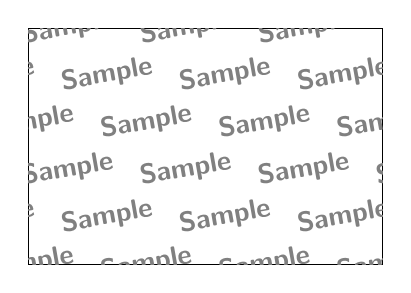
\begin{tikzpicture}
    \draw rectangle++(4.5,3);
    \clip rectangle++(4.5,3);
    \foreach\x in{0,1,2,3,4}{
      \foreach\y in{0,1,2,3,4,5,6}{
        \path(\x*1.5-\y*0.5,\y*0.6)node[rotate=10,text=gray]{\sffamily\bfseries\itshape Sample };
      }
    }
  \end{tikzpicture}
  %% 入れる画像：turtlebot3_world.launch.py を起動したときの Gazebo の画面（六角形の壁の中に柱が並んだ世界と TurtleBot3 Burger）のスクリーンショット
  % eps 画像を貼る場合は includegraphics をお使いください。
  % \includegraphics[width=0.8\linewidth]{simulation/turtlebot3_world.png}
  \caption{Gazebo で TurtleBot3 を起動した様子}
  \label{fig:simulation-tb3}
\end{figure}

別のターミナルで、トピックの一覧を見てみましょう。

\begin{terminal}[シミュレーションのトピックの一覧]
~/ros2_ws$ ros2 topic list
/clock
/cmd_vel
/imu
/joint_states
/odom
/robot_description
/scan
/tf
/tf_static
...
\end{terminal}

\cmd{/scan}（LiDAR）、\cmd{/odom}（オドメトリ）、\cmd{/imu}（IMU）、\cmd{/cmd\_vel}（速度の指令）、\cmd{/tf} などのトピックが、ros\_gz\_bridge や robot\_state\_publisher（\ref{sec:tf-viz-rsp}節）によってパブリッシュされていることがわかります。
シミュレーションの中のロボットも、ROS 2 から見れば、これらのトピックを持ったノードの集まりなのです。

\subsection{キーボードで動かす}

TurtleBot3 には、キーボードで操作するためのノードが用意されています。

\begin{terminal}[TurtleBot3 をキーボードで操作する]
~/ros2_ws$ ros2 run turtlebot3_teleop teleop_keyboard
...
Moving around:
        w
   a    s    d
        x

w/x : increase/decrease linear velocity (Burger : ~ 0.22)
a/d : increase/decrease angular velocity (Burger : ~ 2.84)

space key, s : force stop
\end{terminal}

このターミナルを選んだ状態で \key{W} を押すと前進の速度が上がり、\key{X} で下がります。
\key{A} と \key{D} で回転の速度が変わり、\key{S} か \key{Space} で止まります。
ロボットを動かしながら、\cmd{ros2 topic echo /odom} でオドメトリが変わっていく様子も確かめてみましょう。

\begin{point}[TwistStamped]
  ROS 2 Jazzy の TurtleBot3 は、速度の指令に、\cmd{Twist}（\ref{sec:ros2-concepts-topic}節）ではなく \cmd{geometry\_msgs/msg/TwistStamped} 型を使います。
  \cmd{TwistStamped} は、\cmd{Twist} に、時刻と座標系の名前が入った \cmd{header} を加えたメッセージ型です。
\begin{lstlisting}[numbers=none, xleftmargin=0pt, framexleftmargin=0pt]
std_msgs/Header header      # 時刻（stamp）と座標系の名前（frame_id）
Twist twist                 # 今までの Twist と同じ
\end{lstlisting}
  \cmd{ros2 topic info /cmd\_vel} で、トピックの型を確かめる習慣をつけておきましょう。
\end{point}

\section{センサのシミュレーション}
\label{sec:simulation-sensor}

\subsection{LiDAR}

TurtleBot3 Burger には、周りの物までの距離を、ぐるりと 360 度測る LiDAR が搭載されています。
LiDAR のデータは、\cmd{/scan} トピックに \cmd{sensor\_msgs/msg/LaserScan} 型でパブリッシュされます。
型の中身の主な部分を見てみましょう。

\begin{terminal}[LaserScan 型の中身（一部）]
~/ros2_ws$ ros2 interface show sensor_msgs/msg/LaserScan
std_msgs/Header header
float32 angle_min        # start angle of the scan [rad]
float32 angle_max        # end angle of the scan [rad]
float32 angle_increment  # angular distance between measurements [rad]
...
float32 range_min        # minimum range value [m]
float32 range_max        # maximum range value [m]
float32[] ranges         # range data [m]
...
\end{terminal}

\cmd{ranges} は、測った距離のリストです。
1 つ目の値は \cmd{angle\_min} の向き、2 つ目の値はそこから \cmd{angle\_increment} だけ回った向き……というように、向きを少しずつ変えながら測った距離が並んでいます。
\cmd{range\_min} より近い値や、\cmd{range\_max} より遠い値（何も当たらなかったときは \cmd{inf}）は、正しく測れなかった値として扱います。
\ref{sec:practice-avoid}節では、このデータを読んで障害物を避けるノードを作ります。

\cmd{--once} を付けると、1 回分のメッセージだけを表示できます。
\cmd{ranges} は長いので、\cmd{--field} で見たい部分だけを表示するとよいでしょう。

\begin{terminal}[LaserScan の一部だけを表示する]
~/ros2_ws$ ros2 topic echo --once --field range_max /scan
3.5
---
\end{terminal}

\subsection{RViz2 でセンサのデータを見る}

センサのデータは、数値で見るより、RViz2（\ref{sec:tf-viz-rviz}節）で表示したほうがわかりやすくなります。
\cmd{use\_sim\_time} を \cmd{true} にして RViz2 を起動し、次のように設定してみましょう。

\begin{terminal}[シミュレーションの時刻を使って RViz2 を起動する]
~/ros2_ws$ rviz2 --ros-args -p use_sim_time:=true
\end{terminal}

\begin{enumerate}
  \item 「Fixed Frame」を \cmd{odom} にします。
  \item 「Add」から「RobotModel」を追加し、「Description Topic」を \cmd{/robot\_description} にします。
  \item 「Add」の「By topic」タブから、\cmd{/scan} の「LaserScan」を追加します。
\end{enumerate}

ロボットの周りに、LiDAR が測った点が表示され、柱の形が浮かび上がります。
キーボードでロボットを動かすと、点の見え方が変わっていく様子がわかります。

\subsection{カメラと IMU}

TurtleBot3 Waffle には、カメラも搭載されています。
\cmd{TURTLEBOT3\_MODEL} を \cmd{waffle} にしてシミュレーションを起動すると、カメラの画像が \cmd{sensor\_msgs/msg/Image} 型でパブリッシュされます。
画像は、RViz2 の「Image」の表示か、\cmd{rqt\_image\_view} で見られます。

\begin{terminal}[Waffle でシミュレーションを起動して、カメラの画像を見る]
~/ros2_ws$ TURTLEBOT3_MODEL=waffle ros2 launch turtlebot3_gazebo turtlebot3_world.launch.py
$ ros2 run rqt_image_view rqt_image_view   # 別のターミナルで
\end{terminal}

\cmd{rqt\_image\_view} の画面の左上で、画像のトピック（\cmd{/camera/image\_raw} など）を選ぶと、ロボットから見た景色が表示されます。
コマンドの前に \cmd{変数名=値} を書くと、そのコマンドを実行するときだけ環境変数を設定できます（\ref{sec:env-export-source}節）。

IMU のデータは、\cmd{/imu} トピックに \cmd{sensor\_msgs/msg/Imu} 型でパブリッシュされます。
ロボットの向き（クォータニオン）、角速度、加速度が入っていて、ロボットを回転させると \cmd{angular\_velocity.z} の値が変わります。

\begin{terminal}[IMU のデータを表示する]
~/ros2_ws$ ros2 topic echo --field angular_velocity /imu
\end{terminal}

シミュレーションのセンサにも、設定によっては現実のセンサのような雑音が加えられています。
センサの値が少しずつ揺れるのは、そのためです。
現実のセンサには必ず雑音があるので、それでもうまく動くプログラムを書くことが大切です。

\section*{この章のまとめ}

\begin{itemize}
  \item シミュレーションを使うと、ロボットがなくても、壊す心配なく、何度でもプログラムを試せます。ただし、現実と完全には同じになりません。
  \item ROS 2 Jazzy では、新しい Gazebo（Harmonic）を使います。Gazebo Classic の情報と混同しないように注意しましょう。
  \item ros\_gz\_bridge が、Gazebo と ROS 2 の間でメッセージを中継します。シミュレーションと組み合わせるノードは、\cmd{use\_sim\_time} を \cmd{true} にします。
  \item TurtleBot3 のシミュレーションでは、\cmd{/scan}・\cmd{/odom}・\cmd{/imu}・\cmd{/cmd\_vel} などのトピックで、ロボットとやり取りできます。
  \item LiDAR のデータ（\cmd{LaserScan}）は、向きを少しずつ変えながら測った距離のリストです。RViz2 で表示すると、周りの様子がよくわかります。
\end{itemize}
